\documentclass[11pt]{article}
\usepackage{fullpage}
\usepackage{xcolor}
\usepackage{graphicx}
\usepackage{hyperref}
\usepackage{amsmath}
\usepackage{tikz}
\usetikzlibrary{trees}

\title{Binary Tree Operations Project Documentation}
\author{Jude Eschete}
\date{\today}

\begin{document}
	
	\maketitle
	
	\section{Introduction}
	This document details the design, algorithm, and API of a C++ project that implements various binary tree operations. The functionalities include:
	\begin{enumerate}
		\item Building a binary tree with minimal height.
		\item Validating if the tree is a Binary Search Tree (BST).
		\item Printing all elements in the tree within a given range.
		\item Finding the first common ancestor of two nodes.
	\end{enumerate}
	
	\section{Design and Algorithm}
	
	\subsection{Building a Minimal Height Tree}
	To build a minimal height tree, the algorithm employs a divide-and-conquer strategy by choosing the middle element of a sorted array as the root. This ensures that the left and right subtrees have approximately the same number of nodes.
	
	\textbf{Pseudocode:}
	\begin{verbatim}
		function buildMinimalHeightTree(arr, start, end):
			if start > end:
				return NULL
			mid = start + (end - start) / 2
			node = new Node(arr[mid])
			node.left  = buildMinimalHeightTree(arr, start, mid - 1)
			node.right = buildMinimalHeightTree(arr, mid + 1, end)
			return node
	\end{verbatim}
	
	\subsection{Validating the BST}
	Validation uses a recursive function that checks whether each node's value is within an acceptable range. This range is updated as the recursion traverses down the tree.
	
	\textbf{Pseudocode:}
	\begin{verbatim}
		function validateBSTUtil(node, minVal, maxVal):
			if node is NULL:
				return true
			if node.data < minVal or node.data > maxVal:
				return false
			
			return validateBSTUtil(node.left,  minVal,     node.data - 1) AND
				validateBSTUtil(node.right, node.data + 1, maxVal)
		
		function validateBST(root):
			return validateBSTUtil(root, -infinity, infinity)
	\end{verbatim}
	
	\subsection{Printing Elements in a Given Range}
	If the tree is a BST, an in-order traversal is used to print all nodes whose values lie within a specified range \([k_1, k_2]\).
	
	\textbf{Pseudocode:}
	\begin{verbatim}
		function printRange(node, k1, k2):
			if node is NULL:
				return
		
			if node.data > k1:
				printRange(node.left, k1, k2)
		
			if k1 <= node.data <= k2:
				print node.data
		
			if node.data < k2:
				printRange(node.right, k1, k2)
	\end{verbatim}
	
	\subsection{Finding the First Common Ancestor}
	The function locates the first common ancestor of two nodes by recursively searching both left and right subtrees. If both sides return non-NULL, the current node is the common ancestor.
	
	\textbf{Pseudocode:}
	\begin{verbatim}
		function firstCommonAncestor(node, k1, k2):
			if node is NULL:
				return NULL
			
			if node.data == k1 or node.data == k2:
				return node
			
			left  = firstCommonAncestor(node.left,  k1, k2)
			right = firstCommonAncestor(node.right, k1, k2)
			
			if left != NULL and right != NULL:
				return node
			
			if left != NULL:
				return left
			else:
				return right
	\end{verbatim}
	
	\section{API Specifications}
	
	\subsection{\texttt{buildMinimalHeightTree}}
	\textbf{Prototype:}
	\begin{verbatim}
		Node* buildMinimalHeightTree(const vector<int>& arr, int start, int end)
	\end{verbatim}
	
	\textbf{Description:} Recursively constructs a binary tree with minimal height by choosing the middle element of the array as the root.
	
	\subsection{\texttt{validateBST}}
	\textbf{Prototype:}
	\begin{verbatim}
		bool validateBST(Node* root)
	\end{verbatim}
	
	\textbf{Description:} Uses a recursive helper function to verify that the tree meets BST constraints (left subtree < root < right subtree).
	
	\subsection{\texttt{printRange}}
	\textbf{Prototype:}
	\begin{verbatim}
		void printRange(Node* root, int k1, int k2)
	\end{verbatim}
	
	\textbf{Description:} Prints all elements in the tree within the inclusive range \([k1, k2]\) by performing an in-order traversal optimized for BSTs.
	
	\subsection{\texttt{firstCommonAncestor}}
	\textbf{Prototype:}
	\begin{verbatim}
		Node* firstCommonAncestor(Node* root, int k1, int k2)
	\end{verbatim}
	
	\textbf{Description:} Finds and returns the node that is the first common ancestor of two specified node values.
	
	\section{Example Screenshot and Outputs}
	\includegraphics[width=0.8\textwidth]{images/screenshot1.png}
	
	
	\section{Additional Information}
	\begin{itemize}
		\item \textbf{Input Assumptions:} The array contains unique integers; using a sorted array is recommended.
		\item \textbf{Efficiency:} The divide-and-conquer approach ensures minimal height. BST checks and in-order traversals are implemented recursively.
		\item \textbf{Potential Enhancements:} Additional error handling, iterative methods, and deletion or balancing routines.
	\end{itemize}
	
	\newpage
	
	\subsection*{6.1 Rebalance of the RB-Tree}
	\label{sec:rbfix}
	
	In the intermediate status of the RB-Tree, there was a red-red conflict: node \texttt{P} was red and its child \texttt{N} was also red. This violates the Red-Black property that a red node cannot have a red child. To fix this, we performed the appropriate rotation around the grandparent (\texttt{G}) and recolored nodes to ensure the root remains black and all other RB-Tree properties are maintained (e.g., no consecutive red nodes, equal black height on all paths).
	
	A possible final balanced version of the RB-Tree after rebalancing is shown in Figure~\ref{fig:RBtree61}. Node colors have been updated to remove any red-red violations, and rotations ensure that the tree is properly balanced.
	
	\begin{figure}[h!]
		\centering
		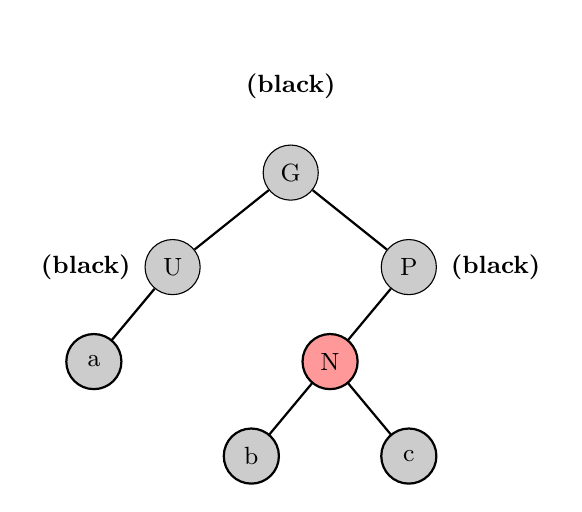
\begin{tikzpicture}[
			level distance=1.2cm,
			every node/.style={draw, circle, font=\small, minimum size=7mm},
			edge from parent/.style={draw, thick},
			level 1/.style={sibling distance=3.0cm},
			level 2/.style={sibling distance=2.0cm},
			>=stealth
			]
			
			% Example final arrangement for 6.1
			\node[fill=black!20,label=above:{\textbf{(black)}}] (G) {G}
			child {
				node[fill=black!20,label=left:{\textbf{(black)}}] (U) {U}
				child {
					node[fill=black!20] (a) {a}
				}
				child[missing] % empty child if needed
			}
			child {
				node[fill=black!20,label=right:{\textbf{(black)}}] (P) {P}
				child {
					node[fill=red!40] (N) {N}
					child {
						node[fill=black!20] (b) {b}
					}
					child {
						node[fill=black!20] (c) {c}
					}
				}
				child[missing]
			};
		\end{tikzpicture}
		\caption{A rebalanced RB-Tree for 6.1, with corrected colors and structure.}
		\label{fig:RBtree61}
	\end{figure}
	
	\noindent
	After these adjustments:
	\begin{itemize}
		\item The root (\texttt{G}) is black, satisfying the property that the root of an RB-Tree is always black.
		\item No red node has a red parent, removing the original red-red conflict.
		\item Every path from the root to a leaf or NULL child has the same number of black nodes, preserving the black-height property.
	\end{itemize}
	
	\newpage
	\subsection*{6.2 Rebalance of the RB-Tree}
	\label{sec:rbfix62}
	
	In the intermediate status for 6.2, a red-red conflict arises because \texttt{P} is red and its child \texttt{N} is also red. This situation violates the Red-Black property that forbids a red node from having a red parent. Additionally, we must ensure that the resulting tree maintains a consistent black height on every path from the root to a leaf (or NULL) child.
	
	To fix this violation, we identify \texttt{G} as the grandparent of \texttt{N}, note that the “uncle” node is black, and perform the appropriate rotation(s) around \texttt{G}. We then recolor the involved nodes to eliminate the red-red conflict while preserving the black-height property. Figure~\ref{fig:RBtree62} shows a possible final arrangement of the tree after these adjustments, with \texttt{P} as the new root and no consecutive red nodes remaining.
	
	\begin{figure}[h!]
		\centering
		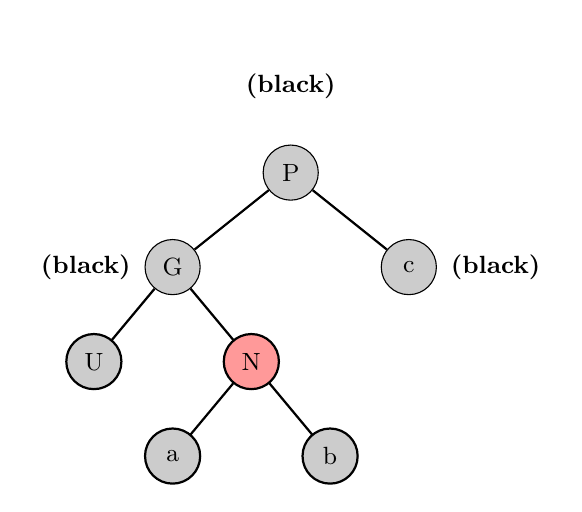
\begin{tikzpicture}[
			level distance=1.2cm,
			every node/.style={draw, circle, font=\small, minimum size=7mm},
			edge from parent/.style={draw, thick},
			level 1/.style={sibling distance=3.0cm},
			level 2/.style={sibling distance=2.0cm},
			>=stealth
			]
			
			% A hypothetical final arrangement after rebalancing 6.2
			\node[fill=black!20,label=above:{\textbf{(black)}}] (P) {P}
			child {
				node[fill=black!20,label=left:{\textbf{(black)}}] (G) {G}
				child {
					node[fill=black!20] (U) {U}
				}
				child {
					node[fill=red!40] (N) {N}
					child {
						node[fill=black!20] (a) {a}
					}
					child {
						node[fill=black!20] (b) {b}
					}
				}
			}
			child {
				node[fill=black!20,label=right:{\textbf{(black)}}] (c) {c}
			};
		\end{tikzpicture}
		\caption{A possible rebalanced RB-Tree for 6.2, with \texttt{P} rotated up and recolored to eliminate the red-red conflict.}
		\label{fig:RBtree62}
	\end{figure}
	
	\noindent
	\textbf{Why These Changes Were Necessary:}
	\begin{itemize}
		\item \textit{Red-Red Conflict:} Before rebalancing, both \texttt{P} and \texttt{N} were red. Rotations and recoloring were required so that a red node (\texttt{N}) would have a black parent (\texttt{P}).
		\item \textit{Maintaining Black-Height:} By adjusting the tree structure and colors, we ensure each path from \texttt{P} to a leaf or NULL pointer has the same number of black nodes.
		\item \textit{Root is Black:} In standard Red-Black Tree rules, the root should be black. Thus, \texttt{P} is recolored to black after the rotation.
	\end{itemize}
	
	
\end{document}
